\documentclass{article}

\PassOptionsToPackage{numbers, compress}{natbib}

\usepackage[main, final]{neurips_2025}

\usepackage[utf8]{inputenc}
\usepackage[T1]{fontenc}
\usepackage{hyperref}
\usepackage{url}
\usepackage{booktabs}
\usepackage{amsfonts}
\usepackage{nicefrac}
\usepackage{microtype}
\usepackage{xcolor}
\usepackage{graphicx}
\usepackage{subcaption}
\usepackage{array}
\usepackage{enumitem}
\usepackage{float}
\usepackage{tikz}
\usetikzlibrary{positioning, arrows.meta, decorations.pathreplacing, calc}

\title{Paper Review: Weak-to-Strong Generalization}

\author{
  Vedant Borkute \\
  Student ID: 862552981
}

\begin{document}

\maketitle

\textbf{Paper title:} Weak-to-Strong Generalization: Eliciting Strong Capabilities with Weak Supervision \\
\textbf{Author(s):} Collin Burns, Pavel Izmailov, Jan Hendrik Kirchner, Bowen Baker, Leo Gao, Leopold Aschenbrenner, Yining Chen, Adrien Ecoffet, Manas Joglekar, Jan Leike, Ilya Sutskever, Jeff Wu (OpenAI) \cite{burns2023weak} \\

% -----------------------------------------------------------------------
\section{Executive Summary}
% -----------------------------------------------------------------------

The paper \cite{burns2023weak} addresses a forward-looking question for alignment: when supervisors can only provide \textit{flawed} labels, can a much stronger pretrained model still recover most of its true capability through finetuning, or does it inevitably collapse to imitating its supervisor's mistakes? This is intended as an empirical analog for the \textit{superalignment} problem, where humans must oversee models whose outputs they cannot reliably evaluate---a regime in which today's reinforcement learning from human feedback (RLHF) pipeline \cite{christiano2017rlhf, ouyang2022instructgpt} is no longer guaranteed to work.

Their principal methodological contribution is the \textit{weak-to-strong} setup itself together with the \textit{Performance Gap Recovered} (PGR) metric. They (i) train a small base model on ground truth to serve as the weak supervisor, (ii) finetune a much larger pretrained model on the weak supervisor's predictions, and (iii) compare against the same large model finetuned on ground truth, which defines the \textit{strong ceiling}. PGR is the fraction of the (weak, strong-ceiling) accuracy gap that weak supervision recovers: PGR$=1$ matches the ceiling, PGR$=0$ matches the supervisor. The setup is run across roughly $7$ orders of magnitude of pretraining compute using base models from the GPT-4 family on three task families: $22$ NLP classification benchmarks, Lichess chess puzzles (generative best-move prediction), and the proprietary ChatGPT reward modeling (RM) dataset.

Their headline result is that \textit{naive} cross-entropy finetuning on weak labels already yields positive PGR almost universally. Supervising GPT-4 with GPT-2-level labels on NLP recovers roughly $50\%$ of the gap on a median task, and PGR often exceeds $50\%$ for the largest students. However, the picture is uneven across task families and the gap to the ceiling is substantial---particularly for reward modeling, where PGR is typically around $10\%$ and rarely exceeds $20\%$, which is exactly the regime closest to RLHF. Figure~\ref{fig:pgr} summarizes the three reference quantities and the PGR definition.

\begin{figure}[H]
  \centering
  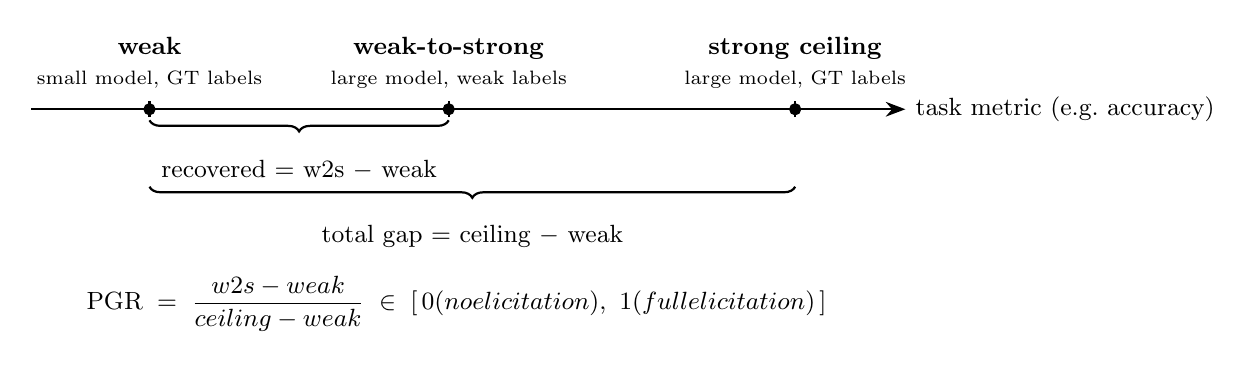
\begin{tikzpicture}[
    >={Stealth[length=2.5mm]},
    every node/.style={font=\small},
  ]
    \def\xw{1.2}
    \def\xs{5.0}
    \def\xc{9.4}

    % main axis
    \draw[->, thick] (-0.3,0) -- (10.8,0) node[right] {\small task metric (e.g.\ accuracy)};

    % markers
    \foreach \x in {\xw, \xs, \xc} \filldraw (\x,0) circle (2pt);
    \foreach \x in {\xw, \xs, \xc} \draw[thick] (\x,-0.10) -- (\x,0.10);

    % labels above each marker
    \node[above=4pt, align=center] at (\xw,0)
      {\textbf{weak} \\ \scriptsize small model, GT labels};
    \node[above=4pt, align=center] at (\xs,0)
      {\textbf{weak-to-strong} \\ \scriptsize large model, weak labels};
    \node[above=4pt, align=center] at (\xc,0)
      {\textbf{strong ceiling} \\ \scriptsize large model, GT labels};

    % short brace below: recovered portion (numerator)
    \draw[decorate, decoration={brace, amplitude=4pt, mirror, raise=4pt}, thick]
      (\xw,0) -- (\xs,0)
      node[midway, yshift=-22pt] {\small recovered $=$ w2s $-$ weak};

    % long brace below: total gap (denominator)
    \draw[decorate, decoration={brace, amplitude=4pt, mirror, raise=28pt}, thick]
      (\xw,0) -- (\xc,0)
      node[midway, yshift=-46pt] {\small total gap $=$ ceiling $-$ weak};

    % PGR formula
    \node[anchor=north, align=center] at (5.1, -2.0)
      {\(\displaystyle
        \mathrm{PGR} \;=\;
        \frac{\text{w2s} - \text{weak}}{\text{ceiling} - \text{weak}}
        \;\in\;[\,\text{0 (no elicitation)},\ \text{1 (full elicitation)}\,]
      \)};
  \end{tikzpicture}
  \caption{Performance Gap Recovered (PGR). All three quantities lie on a common task-metric axis. The \textit{weak} supervisor is a small model finetuned on ground truth, the \textit{strong ceiling} is a large model finetuned on ground truth, and the \textit{weak-to-strong} student is the same large model finetuned on the weak supervisor's labels. PGR measures what fraction of the (weak, ceiling) gap the student recovers; the auxiliary confidence loss, bootstrapping, and unsupervised generative finetuning each shift the weak-to-strong marker rightward in their respective task families.}
  \label{fig:pgr}
\end{figure}

The paper then shows that three simple interventions can substantially improve PGR, each tailored to one task family:
\begin{itemize}[leftmargin=*]
  \item Auxiliary confidence loss on NLP: an additional cross-entropy term that pulls the strong model toward its own hardened predictions when it disagrees with the supervisor, related to conditional entropy minimization \cite{grandvalet2004entropy}. This raises median PGR from $\sim$$25\%$ to $\sim$$80\%$ at the largest weak--strong gaps.
  \item Bootstrapping on chess: a sequence of intermediate-sized students $M_1 \to M_2 \to \dots \to M_n$ where each $M_{i+1}$ is supervised by $M_i$, recovering otherwise-flat scaling curves and aligning with the ``align-slightly-superhuman-first'' alignment plan \cite{leike2018scalable}.
  \item Unsupervised generative finetuning on RM dialog text before preference finetuning: a representation-saliency intervention that adds $10$--$20$ PGR points naively and $30$--$40$ when combined with ground-truth early stopping.
\end{itemize}

A separate set of probing experiments (Section 5.2.3) shows that finetuning on weak labels makes the ground-truth concept \textit{more linearly represented} in the strong model's activations: a linear probe trained with ground truth labels on top of a weakly-finetuned model recovers $\sim$$78\%$ accuracy versus $\sim$$72\%$ from a probe on the base model, closing roughly $60\%$ of the probe--finetune gap. The authors interpret this as evidence that weak supervision's main role is to \textit{elicit} latent capability rather than to teach it, which directly connects the setup to the eliciting-latent-knowledge (ELK) research agenda \cite{christiano2022elk, burns2023ccs}.

% -----------------------------------------------------------------------
\section{Strengths}
% -----------------------------------------------------------------------

\begin{enumerate}[leftmargin=*]

  \item
  The strongest contribution, to me, is the empirical framework itself rather than any single result. Prior work on aligning superhuman systems was largely theoretical---debate, iterated amplification, ELK \cite{irving2018debate, christiano2018amplification, christiano2022elk}---or studied humans supervising current-generation models, which sidesteps the actual difficulty. PGR converts an open-ended question (``how do we oversee systems we cannot evaluate?'') into a quantitative, reproducible target that is computable on any (weak, strong) model pair and any task with a ground-truth split. The asymmetry of weak supervisor vs.\ ceiling is the right unit, because it isolates the alignment-relevant quantity (how much of the strong model's latent capability is being elicited) from absolute task difficulty. This makes scaling laws \textit{for elicitation} possible to study, much as Kaplan-style loss scaling \cite{kaplan2020scaling, hoffmann2022chinchilla} made compute--data tradeoffs concrete in a different context.

  \item
  The auxiliary confidence loss is a minimal, well-motivated intervention that directly targets the imitation failure mode. Naive cross-entropy training pulls the student toward the supervisor's full distribution, errors included. The confidence term in equation (1) replaces the target with a mixture of the weak label and a thresholded version of the model's own prediction, which means the student is rewarded for being confidently right (even against the supervisor) and penalized for being confidently wrong. Empirically, the agreement plots (Section 4.3.2) show exactly what one would hope: on examples where the supervisor is wrong, agreement drops; on examples where it is right, agreement is preserved. The linear-probe diagnostic strengthens this by giving a mechanistic, representation-level explanation---weak finetuning increases linear separability of the ground-truth concept---rather than relying only on output metrics. This pairing of a simple training-time intervention with an interpretable probe is, in my view, the most reusable methodological lesson of the paper.

\end{enumerate}

% -----------------------------------------------------------------------
\section{Weaknesses and Improvements}
% -----------------------------------------------------------------------

\begin{enumerate}[leftmargin=*]

  \item
  The two disanalogies the authors flag in Section 6.1 are acknowledged but not closed, and both push the headline numbers toward optimism. \textit{Imitation saliency}: today's strong models are not pretrained to predict their weak supervisor, so imitation is a representation-distant failure mode; a future superhuman model trained extensively on human-generated data may collapse to imitation far more readily, which is precisely the regime where the framework would fail to detect the problem. \textit{Pretraining leakage}: most of the $22$ NLP tasks plausibly appear in some form in GPT-4-family pretraining, so what looks like ``elicitation of latent capability'' may partly be retrieval of an observed task. The Appendix D AlexNet$\to$DINO experiment \cite{caron2021dino} is a partial fix because DINO never sees classification labels, but it is still a vision setup at a much smaller scale, and the strong model only does linear probing rather than full finetuning. A stronger evaluation would (a) introduce held-out, post-cutoff tasks for which there is provable absence in pretraining, and (b) include a setup where the strong model is pretrained on a corpus that explicitly contains supervisor-like behavior, to stress-test imitation saliency. Without these, extrapolating from current PGR values to superhuman regimes is hard to justify.

  \item
  The fact that each task family needs a \textit{different} ``best method'' (confidence loss for NLP, bootstrapping for chess, generative finetuning for RM) is a sign that the methods are not yet capturing a unified principle of weak-to-strong elicitation---they are three reasonable but disconnected heuristics. Reward modeling, which is closest to the actual alignment use case (and to RLHF \cite{christiano2017rlhf, ouyang2022instructgpt}), is also where PGR is weakest and where the ``best'' fix---unsupervised generative finetuning plus ground-truth early stopping---borrows from labels that will not exist at superhuman scale. I would strengthen the paper by either (a) attempting a method that is \textit{not} GT-early-stop and yet matches its PGR on RM, or (b) testing the existing methods under RL optimization pressure on top of the trained RM, which is the regime in which reward-hacking and Goodharting typically manifest in practice. As reported, the RM section reads more as a warning than as a solution.

\end{enumerate}

% -----------------------------------------------------------------------
\section{Other Comments}
% -----------------------------------------------------------------------

\begin{itemize}[leftmargin=*]

  \item
  The linear-probing result (Section 5.2.3) is, to me, more conceptually important than the headline PGR numbers. If weak finetuning's primary effect is to make the desired concept \textit{linearly readable}, then the framework points to a different deployment story than ``finetune large models with weak labels.'' It instead suggests: use weak labels (or any cheap signal) to \textit{salientize} the concept, then elicit it with a much smaller, simpler, and more auditable mechanism such as a linear probe or a CCS-style consistency search \cite{burns2023ccs}. This is attractive for alignment because probes are far easier to interpret and inspect than a full finetuned model, and they connect naturally to spurious-correlation findings showing that the right concept often \textit{is} linearly accessible if the right invariance is induced \cite{kirichenko2023spurious}.

  The paper also leaves open the question of how to make the framework less reliant on having any ground truth at all. PGR, GT early stopping, and even the ceiling baseline all require labels that, by construction, will not be available for the tasks superalignment actually targets. A natural next step is to develop \textit{label-free} diagnostics for weak-to-strong generalization---e.g., consistency under prompt variation, agreement across independently-trained probes, or inverse-scaling-style stress tests \cite{mckenzie2023inverse}---so that one can rank candidate methods even when the strong ceiling is unmeasurable. Without such diagnostics, the current setup remains a useful empirical playground but does not yet give a deployable recipe.

\end{itemize}

% -----------------------------------------------------------------------
\bibliographystyle{plainnat}
\bibliography{references}
% -----------------------------------------------------------------------

\end{document}
